\chapter{Postulates of Quantum Mechanics}

\section{State Space}

\begin{postulate}
    Any isolated physical system has a Hilbert Space associated with it known as the \textbf{state space}. The system is completely described by it's \textbf{state vector}, which is a unit vector in state space.
\end{postulate}

The simplest quantum mechanical system, which we'll be concerned the most about, is a \textit{qubit} which has a 2-dimensional state space. Hence an arbitrary state vector $\ket{\psi}$ can be represented by

\begin{equation}
    \ket{\psi} = \alpha \ket{0} + \beta \ket{\psi}
\end{equation}

where $\alpha, \beta \in \mathbb{C}$ and $\ket{0}, \ket{1}$ form an orthonormal basis of state space. Since state vector is a unit vector, $\braket{\psi|\psi} = 1 \implies |\alpha|^2 + |\beta|^2 = 1$, this is known as \textit{normalization} of state vector.

For now, \textit{qubit} is an abstract thing. We consider a fixed orthonormal basis $\ket{0}, \ket{1}$ apriori. These two states can be considered analogous to the bits 0 and 1, except that a state vector is a linear combination, or in other words, \textit{superposition } of these bits. The linear combination $\sum_i \alpha_i \ket{\psi_i}$ is defined as the superposition of $\ket{\psi_i}$ with amplitude $\alpha_i$ for $\ket{\psi_i}$.


\section{Evolution}

\begin{postulate}
    The evolution of a \textbf{closed} system is described by a \textbf{unitary transformation}. The state of the system $\ket{\psi}$ at time $t_1$ is related to the state of the system $\ket{\psi^{'}}$ at time $t_2$ solely by the unitary transformation U which only depends on $t_1, t_2$

    \begin{equation}
        \ket{\psi^{'}} = U\ket{\psi}
    \end{equation}
    \label{postulate_2}
\end{postulate}

Quantum mechanics doesn't help us find the \textit{state space} or \textit{unitary operator}, it just assures us that any physical system would behave this way.

Few such operator on a qubit are pauli matrices. X is referred to as \textit{NOT gate} or \textit{bit-flip} since it turns $\ket{0}$ to $\ket{1}$ and vice versa. Z is known as \textit{phase-flip} as it leaves $\ket{0}$ as it is, which inverting the phase (sign) of $\ket{1}$.

The second postulate just defines state of the system at discrete intervals $t_1$ and $t_2$, this can be generalised for \textit{continuous} t.
\begin{corollary}
    Time evolution of a \textbf{closed} quantum system is described by \textbf{Schrödinger equation},
    \begin{equation}
        i\hbar \frac{d\ket{\psi}}{dt}
        = H\ket{\psi}
    \end{equation}
    where $\hbar$ is the reduced planck's constant, H is a fixed \textbf{Hermitian} operator known as the \textbf{Hamiltonian} of the closed system.
    \label{schrodinger_eq}
\end{corollary}

Since Hamiltonian is a Hermitian operator, it has a spectral decomposition,
\begin{equation}
    H = \sum_E E\ket{E}\bra{E}
\end{equation}

Here the eigenvectors $\ket{E}$ are conventionally called \textit{energy eigenstates} or \textit{stationary states} and $E$ is called \textit{energy} of the state $\ket{E}$. The lowest energy is known as \textit{ground state energy} and the corresponding state is the \textit{ground state.}

We can see a connection between corollary \ref{postulate_2} and postulate \ref{schrodinger_eq}, if we know the solution of Schr\"{o}dinger's equation, which can be verified that it is

\begin{equation}
    \ket{\psi(t_2)} = exp\left[\frac{-iH(t_2-t_1)}{\hbar}\right]\ket{\psi(t_1)} = U(t_1,t_2)\ket{\psi(t_1)}
\end{equation}

if we set, 
\begin{equation}
    U(t_1,t_2) \equiv exp\left[\frac{-iH(t_2-t_1)}{\hbar}\right]
\end{equation}

it can be shown that if $K$ is a Hermitian operator, then $U=exp(iK)$ is a unitary operator. Thus, there's a one-to-one correspondence between the theorem and it's corollary.

If the system we're considering is not closed, we can approximate it's evolution using a time varying Hamiltonian. There's this example that when we consider a laser focused on an atom, the whole system is properly described by a Hamiltonian, but the behaviour of the atome alone, is seem to be approximately described by another Hamiltonian, this thing contains terms related to the laser intensity.

\section{Quantum measurement}

We've seen that in closed systems, the evolution of state vector is according to a unitary transform, but when we try to measure the state of the system, we need to interact with it, which leads to a change other than a unitary transform, which is described as

\begin{postulate}
    A \textbf{quantum measurement} is a collection $\{M_m\}$ of measurement operators. These operators act on the state space. The index m refers to the measurement outcome that we want using $M_m$. If the system is in state vector $\ket{\psi}$ before the measurement had been made, the probability that outcome is m is,
    \begin{equation}
        \label{eq:measurement_probability}
        p(m) = \bra{\psi}M_m^\dag M_m\ket{\psi}
    \end{equation}
    After the measurement, the state changes to
    \begin{equation}
        \frac{M_m\ket{\psi}}{\sqrt{\bra{\psi}M_m^\dag M_m\ket{\psi}}}
    \end{equation}
    All the $M_i$ satisfy the \textbf{completeness relation}
    \begin{equation}
        \sum_i M_i^\dag M_i = I
    \end{equation}
    This ensures the probability that some measurement occurs is 1,
    \begin{equation}
        \sum_i p(i) = \sum_i \bra{\psi}M_i^\dag M_i\ket{\psi} = 1
    \end{equation}
\end{postulate}

As an example, suppose we have a closed system whose state vector $\ket{\psi}$ is currently $a\ket{0} + b\ket{1}$ and we want to make measurements using $M_0 = \ket{0}\bra{0}$ and $M_1 = \ket{1}\bra{1}$, we can calculate and see that probability that measurements 0 \& 1 are made correct are $|a|$ and $|b|$ respectively, and the final states are
$\frac{a}{|a|}\ket{0}$ if we make measurement 0 and $\frac{b}{|b|}\ket{1}$ if we make measurement 1.

So when there's an isolated physical system, it has a state vector, when you try to measure it, using the collection of measurement operators gives just a label. we can just get the probability that we get a specific probability, using equation \ref{eq:measurement_probability}

\section{Distinguishing quantum states}
When we have $n$ systems, with $n$ state vectors, we can only distinguish them by measuring them only if all the state vectors are orthonormal. This has a good proof.

\begin{theorem}
    No measurement distinguishing non-orthogonal states is possible
\end{theorem}

\begin{proof}
    We consider two states $\ket{\psi_1}, \ket{\psi_2}$ and assume that there exists a measurement. We distinguish these states by looking at the output label we get from the measurement. Taking the function $f(j)$ where $j$ is the label. If the state is $\ket{\psi_1}$ then probability that our prediction is correct $\sum_{j; f(j)=1} \bra{\psi_1}M_j^\dag M_j \ket{\psi_1} = 1$ similarly for 2. To simlify this we define

    \begin{equation}
        E_i = \sum_{j; f(j) = i} M_j^\dag M_j
    \end{equation}
    so from what we've done above
    \begin{align}
        \bra{\psi_1}E_1\ket{\psi_1} = 1 &
        \bra{\psi_2}E_2\ket{\psi_2} = 1
    \end{align}
    since we'll always measure $\ket{\psi_1}$'s label when the state is $\ket{\psi_1}$,
    \begin{align}
        \bra{\psi_1}E_2\ket{\psi_2} &= 0 \\
        \implies \sqrt{E_2}\ket{\psi_2} &= 0
    \end{align}
    now let's focus on the orthogonal component of $\ket{\psi_2}$, by writing it as $\ket{\psi_2} = \alpha \ket{\psi_1} = \beta \ket{\phi}$, where $\ket{\phi}$ is orthonormal to $\ket{\psi_1} \implies 
    |\beta| < 1$, since they're non-orthogonal.

    But there's a contradiction,
    \begin{align}
        \bra{\psi_2}E_2\ket{\psi_2} &=
        \beta^2 \bra{\phi}E_2\ket{\phi} \\
        &\leq |\beta|^2 \\
        &< 1 
    \end{align}
    Thus by contradiction, our assumption is false $\implies$ we can't distinguish non-orthogonal states reliably.
\end{proof}

\section{Projective measurements}
This is the main thing we'll deal in quantum information and computation.

\begin{postulate}
    A projective measurement is an observable M, a Hermitian operator on the state space of system considered, having spectral decomposition
    \begin{equation}
        M = \sum_m mP_m
    \end{equation}
    where m is one of the possible outcomes. m is an eigenvalue of $M$, $P_m$ is the projector onto the corresponding eigenspace. When we measure a state $\ket{\psi}$, the probability of getting the result m is
    \begin{equation}
        p(m) = \bra{\psi}P_m\ket{\psi}
    \end{equation}
    After measuring, the state of the system becomes
    \begin{equation}
        \frac{P_m\ket{\psi}}{\sqrt{p(m)}}
    \end{equation}
\end{postulate}

We can see projective measurement is a special kind of measurement, which do obey completeness relation, i.e $\sum_m M_m^\dag M_m = I$. But $M_m$ also are \textit{Orthogonal projectors}, hence \textit{Hermitian} and $M_mM_{m^`} = \delta_{mm^`}M_m$

These have few nice properties, we can find mean of measurements easily, which is
\begin{align}
    E(M) &= \sum_m m p(m) \\
    &= \sum_m m\bra{\psi} P_m \ket{\psi} \\
    &= \bra{\psi} \sum_m mP_m \ket{\psi} \\
    &= \bra{\psi}M\ket{\psi}
\end{align}

this is a nice thing, we can also find the standard deviation of the outcomes we get.

\begin{align}
    \Delta(M) &= \sqrt{\braket{(M-\braket{M}}^2} \\
    &= \sqrt{\braket{M^2} - \braket{M}^2}
\end{align}

As you might have observed, we defined a new term \textit{observable}, some still like to look at the projection measurement as a collection of operators, using the observable implicitly. Another phrase used is "measure in basis $\ket{m}$", which means the projectors $P_m = \ket{m}\bra{m}$ are used for projective measurement.

If $\vv{v}$ be a three dimensional unit vector, then the measurement of the observable
\begin{equation}
    \vv{v}\cdot \vv{\sigma} = v_1\sigma_1 + v_2\sigma_2 + v_3\sigma_3
\end{equation}
is historically known as the "\textit{measurement of spin along $\vv{v}$ axis}"

\begin{remark}
    Eigenvalues of $\vv{v}\cdot\vv{\sigma}$ are $\pm 1$ and the corresponding projection operators are $P_{\pm} = \frac{I \pm \vv{v}\cdot\vv{\sigma}}{2}$
\end{remark} 

\subsection{Heisenberg Uncertainty Principle}
Suppose $A$, $B$ be two Hermitian operators and $\ket{\psi}$ is a quantum state. Let $\bra{\psi}AB\ket{\psi} = x+iy$ where $x, y \in \mathbb{R}$. Then $\bra{\psi}[AB]\ket{\psi} = 2iy$ and $\bra{\psi}\{AB\}\ket{\psi} = 2x$, therefore

\begin{equation}
    \left( \bra{\psi}[A,B]\ket{\psi} \right)^2 + 
    \left( \bra{\psi} \{A,B\} \ket{\psi} \right)^2 = 
    4\left| \bra{\psi} AB \ket{\psi} \right|^2
\end{equation}
Using Cauchy-Schwartz inequality, then substituting $A = C - \braket{C}$ and $B = D-\braket{D}$
\begin{align}
    \inbk{A^2}\inbk{B^2} &\geq \left(\inbk{AB}\right)^2 \\
    &\geq \frac{\left( \inbk{[A, B]} \right)^2}{4} \\
    \implies \Delta(C)\Delta(D) &\geq
    \frac{\inbk{[C, D]}}{2}
\end{align}
Hence Proved.

Note that the common misconception of Heisenberg uncertainity principle is
that we "measure a state with some error" which is $\Delta(C), \Delta(D)$, but the actual thing is we have a large amount of $\qv$'s and we measure each of them seperately to with observables $C, D$ to get a set of values of $C, D$ whose standard deviation is $\Delta(C), \Delta(D)$. This is because once we make a measurement, the quantum state changes because we've altered it.

\section{POVM measurements}
It stands for \textit{Positive Operator-Valued Measure}. POVM is a formalism, and is used when we are concerned with the outcome more than the state of the output we're measuring. For eg. when we've done an experiment and just want to measure the final state.

If we're measuring a state $\qv$ using measurement operators $M_m$, the probability that the output is $m$ is $\inbk{M_m^\dag M_m}$, if we define
\begin{equation}
    E_m = M_m^\dag M_m
\end{equation}
$E_m$ satisfy $\sum_m E_m = I$, $E_m$ is enough to find the probability of output $m$
which is $\inbk{E_m}$. The set $\{E_m\}$ is called the \textit{POVM set}.

In projective measurements POVM set is same as the set of measurement operators, since $E_m = P_m^\dag P_m = P_m$. In fact any measurement where the measurement operators and the POVM elements coincide is a projective measurement.

If we want the post-measurement state, we can conveniently \textit{define} a POVM to be any set of operators $\{E_m\}$ such that \begin{enumerate*}[label=(\alph*)]
    \item each $E_m$ is positive
    \item it satisfies \textit{completeness relation}, i.e $\sum_m E_m = I$
\end{enumerate*}
In this way we can choose $M_m = U_m\sqrt{E_m}$ where $U_m$ is a unitary operator.

\section{Phase}
This is kind of interesting and deja vu giving.
\subsection{Global Phase}
If $\qv$ is a state, $\theta \in \mathbb{R}$, we say that $e^{i\theta}\qv$ is equal to $\qv$ upto the \textit{global phase factor $e^{i\theta}$}. These two act quite similar when you try to measure them, because the output of m would occur with a probability of $\inbk{M_m^\dag M_m}$ and $\inbk{e^{-i\theta}M_m^\dag M_m e^{i\theta}} = \inbk{M_m^\dag M_m}$, which is the same.
Thus, they're physically equivalent.

\subsection{Relative Phase}
If two amplitudes, $a$ and $b$, \textit{differ by a relative phase} if there is a real $\theta$ such that $a = be^{i\theta}$. Two states \textit{differ by a relative phase} in \textit{some basis} if each of the amplitudes in that basis is related by such a phase factor.
Unlike global phase factors, relative phase factors differ from amplitude to amplitude, thus, there are physically observable differences in measurement statistics, and two states differing by a relative phase aren't physically equivalent.

\section{Composite systems}
It's useful in describing state of a composite system made up of multiple systems 

\begin{postulate}
    The state space of a composite physical system is the tensor product of state spaces of component physical systems. If n physical systems are prepared in state $\ket{\psi_1},\cdots,\ket{\psi_n}$
    The composite system has the state $\ket{\psi_1}\otimes\ket{\psi_2}\otimes\cdots\otimes\ket{\psi_n}$
\end{postulate}

Using this, we can prove a fact.
\begin{remark}
    To implement a general measurement, it is sufficient to make projective measurements together with unitary dynamics
\end{remark}
I'm not giving the entire proof. but assume that the state space we're considering is $Q$ and we want to measure using operators $M_m$. We can consider a new \textit{ancilla} system which has state space $M$. $M$ has orthonormal basis $\ket{m}$ which are in one-to-one correspondence with the first output. Let's define an operator $U:QM \xrightarrow{} QM$ as
\begin{equation}
    U\qv\ket{0} = \sum_m M_m\qv\ket{m}
\end{equation}
where $\ket{0}$ is some state in $Q$. It can be shown that $U$ preserves dot product. i.e $\bra{0}\bra{\phi}U^\dag U \qv\ket{0} = 
\braket{\phi | \psi}$ which implies that U extends over $Q\otimes M$ which can be proved too.

Now, if we consider two systems with projectors $P_m = I_Q\otimes \ket{m} \bra{m}$ and measure using unitary dynamics and projective transformation, the probability of output $m$ is
\begin{align}
    p(m) &= \bra{\psi}\bra{0}U^\dag P_m U \ket{0}\ket{\psi} \\
    &= \sum_{m', m''}\bra{\psi}\bra{m'}M_{m'}^\dag (I_Q \otimes \ket{m}\bra{m})M_{m''}\ket{m''}\ket{\psi}\\
    &= \braket{\psi|M_m^\dag M_m | \psi}
\end{align}
which is just as measured directly from general measurement.
also the state of the composite system after the measurement is
\begin{align}
    \frac{P_mU\ket{\psi}\ket{0}}{\sqrt{\braket{
    \psi | U^\dag P_m U | \psi}
    }}
    =
    \frac{M_m\ket{\psi}\ket{m}}{
    \sqrt{
    \braket{\psi|M_m^\dag M_m | \psi}
    }
    }
\end{align}
Since the state of the system M after measurement is $\ket{m}$, state of system Q is
\begin{align}
    \frac{M_m\ket{\psi}}{\sqrt{
    \braket{\psi|M_m^\dag M_m | \psi}
    }}
\end{align}
also as measured directly from general measurement.

\subsection*{Quantum Entanglement}
This is something you would've heard of before. Consider the two qubit state,
\begin{align}
    \qv = \frac{\ket{00} + \ket{11}}{\sqrt{2}}
\end{align}
we can never write it as a tensor product of two other qubit states, i.e $\qv = \ket{a}\ket{b}$ can never be true. It's easily checkable. A state of a composite system like this, which can't be written as tensor product of it's component systems is an \textit{entangled} state. Entangled states play a cruicial rules in quantum computation and information.

\section{Application: Superdense Coding}
This nicely uses the idea of entanglement and "applying" quantum gates.
Suppose we have 'Alice' and 'Bob' again, who're away from each other. Alice wants two share two classical bits of information using one qubit to bob, can she do it?

\begin{center}
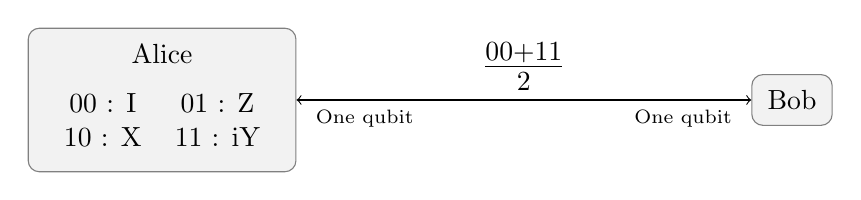
\begin{tikzpicture}
[
place/.style = {rectangle,draw=black!50,fill=black!5,
inner sep=2mm, rounded corners}
]
 \node[place] (alice) at (-4,0)  {
 \begin{minipage}{3cm}
 \centering
 Alice \\
 \vspace{3mm}
 \begin{tabular}{cc}
     00 : I & 01 : Z \\ 
     10 : X & 11 : iY
 \end{tabular}
 \end{minipage}
 };
 \node[place] (bob) at (4,0) {Bob};
 \draw [<->] (alice) -- (bob) node[midway, above] {\Large$
 \frac{\ket{00}+\ket{11}}{2}
 $}
 node[pos = 0.15, below] {
 \scriptsize
   One qubit
 }
 node[pos = 0.85, below] {
   \scriptsize
   One qubit
 };
\end{tikzpicture}
\end{center}

Yes, using superdense coding. Here, Alice and Bob share a pair of externally setup qubits in entangled state
\begin{equation}
   \qv =  \frac{\ket{00}+\ket{11}}{2}
\end{equation}
Alice has one qubit, which she can alter and Bob has another. Any change Alice makes to her qubit changes the composite system, which can be measured by Bob. So she applies quantum gates to change the qubits, as given in the diagram, which result in the following changes.

\begin{align}
    00 &: \qv \xrightarrow{I} \frac{\ket{00}+\ket{11}}{2} \\
    01 &: \qv \xrightarrow{Z}
    \frac{\ket{00}-\ket{11}}{2} \\
    10 &: \qv \xrightarrow{X}
    \frac{\ket{10}+\ket{01}}{2} \\
    11 &: \qv \xrightarrow{iY}
    \frac{-\ket{10}+\ket{01}}{2}
\end{align}

We can see that all the outputs are orthonormal, hence Bob can choose appropriate measurement operators and clearly distinguish each state, hence getting the information Alice had sent him.
These are known as the \textit{Bell states, Bell basis} or \textit{EPR pairs}.

Thus, a single qubit can be used to transfer information which would've taken two classical bits.

\section{The density operator}
Till now we've been using the language of state vectors. The density operator is a different way of representing states, it's mathematically equivalent to state vectors. It's much more convenient to use in some scenarios. It's really useful while describing \textit{individual subsystems} of a composite system.

\subsection{Ensembles of quantum states}
It's useful when we don't exactly know the state of a system. If the possible states are $\ket{\psi_i}$ with probabilities $p_i$, $\{p_i, \ket{\psi_i}\}$ is an \textit{ensemble of pure states}. The density operator, also called as the \textit{density matrix} is defined as
\begin{equation}
    \rho \equiv \sum_i p_i \op{\psi_i}
\end{equation}

We can now workout rewriting the postulates of quantum mechanics. 

Suppose, the evolution of closed quantum system is described by a unitary operator $U$. The system is initially in the state $\ket{\psi_i}$ with probability $p_i$, after the evolution, system will be in the state $U\ket{\psi_i}$ with probability $p_i$, then the density operator evolves into

\begin{equation}
    \rho = \sum_i p_i\op{\psi_i} 
    \xrightarrow{U}
    \sum_i p_i U\op{\psi_i}U^\dag
    = U\rho U^\dag.
\end{equation}

We can also predict the probability of a measurement outcome $m$, when our system is defined by the density operator $\rho$, if the initial state was $\ket{\psi_i}$, then the probabililty of outcome $m$ is

\begin{equation}
    p(m|i) = \braket{\psi_i |M_m^\dag M_m| \psi_i}
    = \text{tr}(M_m^\dag M_m \op{\psi_i})
\end{equation}

This is the probability that the outcome would be $m$, if the state was $\ket{\psi_i}$ which has a probability of $p_i$, hence the overall probability of outcome being m is
\begin{align}
    p(m) &= \sum_i p(m|i)p_i \\
    &= \sum_i p_i\text{tr}(M_m^\dag M_m\op{\psi_i}) \\
    &= \text{tr}(M_m^\dag M_m \rho)
\end{align}
Also we can find out the state of the system if the outcome was m, if the state was initially $\ket{\psi_i}$ which has probability $p_i$ the final state would be
\begin{equation}
    \ket{\psi_i^m} = \frac{M_m\ket{\psi_i}}{
    \sqrt{\braket{\psi_i | M_m^\dag M_m | \psi_i}}
    }
\end{equation}
Hence, the final density operator would be
\begin{equation}
    \rho_m = \sum_i p(i|m)\op{\psi_i^m} = 
    \sum_i p(i|m)\frac{M_m\op{\psi_i}M_m^\dag}{\braket{
    \psi_i| M_m^\dag M_m |\psi_i
    }}
\end{equation}
By Bayes' theorem, $p(i|m) = p(m|i)p_i/p(m)$, subsituting this,
\begin{align}
    \rho_m &= \sum_i p_i \frac{M_m\op{\psi_i}M_m^\dag}{\text{tr}(M_m^\dag M_m \rho)} \\
    &= \frac{M_m\rho M_m^\dag}{\text{tr}(M_m^\dag M_m \rho)}
\end{align}

A system whose state $\qv$ is exactly known is said to be in \textit{pure state}. The density operator is then simply $\op{\psi}$. Otherwise, the system is said to be in a \textit{mixed state}. It's said to be in a \textit{mixture} of different states in the ensemble of $\rho$. Suppose a quantum state is prepared from $\rho_i$ with probability $p_i$, the system can then be described by the density operator $\sum_i p_i\rho_i$, which can be proved.

This is useful in mainly in the analysis of quantum noise, when we need to introduce ignorance into our knowledge of the quantum state. For example if we made a measurement and somehow lost/forgot our measurement, then the final state of the system would be \textit{mixed}, given by
\begin{align}
    \rho &= \sum_m p(m)\rho_m \\
    &= \sum_m \text{tr}(M_m^\dag M_m \rho)
    \frac{M_m\rho M_m^\dag}{\text{tr}(M_m^\dag M_m \rho)} \\
    &= \sum_m M_m \rho M_m^\dag
\end{align}

\section{General properties of density operator}
We can actually characterize what operators are density operators using

\begin{theorem}[\textbf{Characterization of density operators}]
    An operator $\rho$ is a density operator associated with an ensemble $\{p_i, \ket{\psi_i}\}$ if and only if
    \begin{enumerate}
        \item \textbf{Trace condition} $\text{tr}(\rho) = 1$
        \item \textbf{Positivity condition} $\rho$ is a positive operator.
    \end{enumerate}
\end{theorem}
\begin{proof}
    Forward is easy and upto the reader. For the backward proof, a possible ensemble is $\{ \lambda_i, \ket{i}\}$, where $\lambda_i, \ket{i}$ are eigenvalues are corresponding eigenvectors of $\rho$, it's upto the reader to check other conditions.
\end{proof}

With this in our hands, we can redefine our postulates with this density operator picture 
\begin{postulate*}
    Every physical system is associated with a Hilbert space known as it's \textit{state space}. The system is completely described by it's \textit{density operator}, $\rho$ which is a positive operator with trace equal to one acting on the state space of the system. If the system is in state $\rho_i$ with probability $p_i$, the density operator of the system is $\sum_i p_i\rho_i$.
\end{postulate*}

\begin{postulate*}
    The evolution of a \textit{closed} system is described by a \textit{unitary transformation}, i.e state of the system $\rho$ at time $t_1$ is related to the state $\rho'$ at time $t_2$ by a unitary operator which only depends on $t_1$ and $t_2$.
    \begin{equation}
        \rho' = U\rho U^\dag
    \end{equation}
\end{postulate*}

\begin{postulate*}
    A quantum measurement is described by a set  $\{M_m\}$ of \textit{measurement operators}. These act on the state space of the system. The index $m$ refers to the possible outcome of the measurement. If the state of the system is $\rho$ just before the measurement, the probability of outcome $m$ is
    \begin{equation}
       p(m) = \text{tr}(M_m\rho M_m^\dag)
    \end{equation}
    The state of the system changes after the measurement is made, to $\rho'$, given by
    \begin{equation}
        \rho' = \frac{M_m\rho M_m^\dag}{\text{tr}(M_m\rho M_m^\dag)}
    \end{equation}
    The measurement operators satisfy the relation
    \begin{equation}
       \sum_m M_m M_m^\dag = I.
    \end{equation}
\end{postulate*}

\begin{postulate*}
    State space of a composite system is the tensor product of it's component systems. If the components are prepared in state $\rho_1, \rho_2, \cdots, \rho_n$, state of the composite system is given by $\rho_1\otimes \rho_2 \otimes \cdots \otimes \rho_n$.
\end{postulate*}

\begin{remark}
    If $\rho$ is a density operator, then $\tr{\rho^2} \leq 1$. Equality holds when $\rho$ is a pure state.
\end{remark}

By now, you would've noticed that two \textit{different} states can have the same density operator. To get to know what kind of connection there is between these states, we define $\tilde{\ket{\psi_i}}$ associated with the state $\ket{\psi_i}$, the latter is said to \textit{generate} the density operator if $\rho = \sum_i \op{\tilde{\psi_i}}$. It's observable that $\ket{\tilde{\psi_i}} = \sqrt{p_i}\ket{\psi_i}$. Now we proceed for the theorem.

\begin{theorem}[Unitary freedom in the ensemble of the density matrices.]
    Two sets $\Tilde{\ket{\psi_i}}$ and $\tilde{\ket{\phi_j}}$ generate the same density operator if
    \begin{equation}
        \tilde{\ket{\psi_i}} = 
        \sum_j u_{ij}\tilde{\ket{\phi_j}}
    \end{equation}
    where $u_{ij}$ is a unitary matrix. The sets which is smaller is padded with 0.
\end{theorem}

In other words, if they two systems have possible states $\ket{\psi_i}$ and $\ket{\phi_j}$ with probabilities $p_i$ and $q_j$ respectively, they both have the same density operator if and only if
\begin{equation}
    \sqrt{p_i}\ket{\psi_i} = 
    \sum_j u_{ij}\sqrt{q_j}\ket{\phi_j}
\end{equation}
where $u_{ij}$ is a unitary matrix, and the smaller set is padded with 0.

\section{Reduced Density Operator}
This is most useful in describing \textit{subsystems} of a composite quantum system. Suppose we have physical system $A$ and $B$, whose state is described by the density operator $\rho^{AB}$. The reduced density operator for system A is defined by
\begin{equation}
    \rho^A \equiv \text{tr}_B(\rho^{AB}),
\end{equation}
where $\text{tr}_B$ is a map of operators known as the \textit{partial trace} over system $B$. It's defined by
\begin{equation}
    \text{tr}_B(\ket{a_1}\bra{a_2}\otimes\ket{b_1}\bra{b_2}) \equiv \ket{a_1}\bra{a_2}\tr{\ket{b_1}\bra{b_2}},
    \label{eq:partial_trace}
\end{equation}
This partial trace operation is defined only on a special subclass of operators on $AB$; the specification is completed by requiring in addition to Equation (\ref{eq:partial_trace}) that the partial trace be linear in its input.

Let's do an example to understand this better, suppose $\rho^{AB} = \rho \otimes \sigma$, where $\rho$ is the density operator for system A, and $\sigma$ for system B. Then
\begin{equation}
    \rho^{A} = \text{tr}_B(\rho \otimes \sigma) = \rho \tr{\sigma} = \rho
\end{equation}
Which is intuitively correct. For an unintuitive example, let's take an entangled state which would further reveal many things. Let's take the bell state $AB$ $\frac{\ket{00} + \ket{11}}{2}$, which is an entangled state and has the density operator
\begin{align}
    \rho^{AB} &= \left(
        \frac{\ket{00} + \ket{11}}{2}
    \right) \left(
        \frac{\bra{00} + \bra{11}}{2}
    \right) \\
    &= \frac{
    \op{00} + \ket{11}\bra{00} + \ket{00}\bra{11} + \op{11}
    }{2}
\end{align}
Thus we can get $\rho^B$ from this
\begin{align}
    \rho^B &= \text{tr}_A(\rho^{AB}) \\
    &= \frac{
    \tr{\op{0}}\op{0}
    + \tr{\ket{1}\bra{0}}\ket{1}\bra{0}
    }{2}
    \\
    &+ \frac{
     \tr{\ket{0}\bra{1}}\ket{0}\bra{1}
    + \tr{\op{1}}\op{1}
    }{2}
    \\
    &= \frac{
    \op{0} + \op{1}
    }{2}
    \\ &=
    \frac{I}{2}.
\end{align}

This is actually a \textit{mixed state}, since $\tr{(I/2)^2} < 1$. It's wonderful how we can't find state vector of an entangled qubit, but we can find out the density operator of an entangled qubit. Also the composite system is in pure state, but the entangled qubit is in a mixed state, we don't know exactly what it is. This is a really strange property, we can know the exact state of a joint system, but still we can't figure out each subsystem's state exactly. A hallmark of quantum entanglement.

A physical justification for making such an identification is that the reduced density operator provides the correct measurement statistics for the measurements made on system A.

\section{Schmidt decomposition and purifications}
\subsection{Schmidt decomposition}
This is a tool like density operator which are useful for the study of composite quantum systems.
\begin{theorem}[\textbf{Schmidt decomposition}]
    Suppose $\qv$ is a pure state of a composite system, $AB$. Then there exist orthonormal state $\ket{i_A}$ for system A, and orthonormal states $\ket{i_B}$ of system $B$ such that
    \begin{equation}
        \qv = \sum_i \lambda_i \ket{i_A}\ket{i_B},
    \end{equation}
    where $\lambda_i$ are \textbf{non-negative real} numbers satisfying $\sum_i \lambda_i^2 = 1$ known as the \textbf{Schmidt co-efficients}.
\end{theorem}
Do note that it's not the linear combination of all possible tensor product of bases of $A$ and $B$. It's just $i$, i.e linear. Only the tensor product of corresponding bases. This result is very useful. Let $\qv$ be a pure state of a composite system, $AB$. Then by Schmidt decomposition, $\rho^A = \sum_i \lambda_i^2 \op{i_A}$ and $\rho^B = \sum_i \lambda_i^2 \op{i_B}$. Thus eigenvalues of $\rho^A$ and $\rho^B$ are identical, namely $\lambda_i^2$ for both density operators.

\begin{proof}
    We'll consider when $A$ and $B$ have same dimension, it's also true when they're not of same dimension. Let $\ket{j}$ and $\ket{k}$ be fixed o.n.b for $A$ and $B$ respectively, then $\qv$ can be written as
    \begin{equation}
        \qv = \sum_{jk} a_{jk}\ket{j}\ket{k},
    \end{equation}
    where $a_{jk}$ form a matrix $a$. By singular value decomposition, $a = udv$, where $d$ is a diagonal matrix with non-negative elements, $u$ and $v$ are unitary matrices. Thus
    \begin{equation}
        \qv = \sum_{ijk} u_{ji}d_{ii}v_{ik}  \ket{j}\ket{k},
    \end{equation}
    If we define, $\ket{i_A} \equiv \sum_j u_{ji}\ket{j},$ $\ket{i_B} \equiv \sum_k v_ik \ket{k},$ and $\lambda_i \equiv d_{ii}$, it gives
    \begin{equation}
        \qv = \sum_i \lambda_i \ket{i_A}\ket{i_B}
    \end{equation}
    $\ket{i_A}$ and $\ket{i_B}$ form an orthonormal set, from the unitarity of $u$ and $v$ and the orthonormality of $\ket{j}$ and $\ket{k}.$
\end{proof}

\begin{remark}
    If $\ket{ABC}$ is a three component quantum system. There are quantum states $\qv$ of the system which can't be written as
    \begin{equation}
        \qv = \sum_i \lambda_i \ket{i_A}\ket{i_B}\ket{i_C},
    \end{equation}
    where $\lambda_i \in \mathbb{R}$ and $\ket{i_A}, \ket{i_B}, \ket{i_C}$ are the orthonormal bases of the respective systems.
\end{remark}

The bases $\ket{i_A}$ and $\ket{i_B}$ are known as the \textit{Schmidt bases} of systems $A$ and $B$. The number of non-zero values $\lambda_i$ is known as the \textit{Schmidt number} of state $\qv$. It in some sense relates to the "amount" of entanglement in $\qv$. Schmidt number is preserved under unitary transformation, i.e Schmidt number of $U\qv = $ Schmidt number of $\qv$, since $U\qv = \sum_i \lambda_i (U\ket{i_A})\ket{i_B}$.

\subsection{Purification}
Suppose we're given a state $\rho^A$ of a quantum system $A$, which might be \textit{mixed} or \textit{pure}. We can surely introduce a new system R and define a \textit{pure state $\ket{AR}$} for $AR$ such that $A = \text{tr}_R(\op{AR})$. Here $R$ is known as the \textit{reference system} has no physical significance, we just introduced it to \textit{purify} our mixed state, i.e associate our mixed state with a pure state. This thing is known as \textit{purification} of $\rho^A$.

To prove this, suppose $\rho^A$ has the orthonormal decomposition $\sum_i p_i \op{i^A}$. We now introduce a system $R$ which has the same state space as $A$, and has an orthonormal basis $\ket{i^R}$, to define a pure state of the combined system $AR$,
\begin{equation}
    \ket{AR} \equiv \sum_i \sqrt{p_i}\ket{i_A}\ket{i_R}
\end{equation}
Now the reduced density operator of system $A$, corresponding to the state $\ket{AR}$ is
\begin{align}
    \text{tr}_R(\op{AR}) &= \sum_{ij} \sqrt{p_ip_j} \ket{i^A}\bra{j_A}\tr{\ket{i^R}\bra{j^R}} \\
    &= \sum_{ij} \sqrt{p_ip_j} \ket{i^A}\bra{j_A} \delta_{ij} \\
    &= \sum_i p_i \op{i^A} \\
    &= \rho^A
\end{align}
Thus, $\ket{AR}$ is the purification of $\rho^A$.